\subsection{From scan to knot: an interface picture}
\label{subsec:scan_to_knot}

Figure~\ref{fig:hilbert_knot_triptych} provides a narrative visualization of the interface picture used throughout this paper.
The primitive description is a single sequential readout stream (Axiom~\ref{ax:readout_sequentiality}), while spatial language enters only after choosing an addressing basis that folds the stream into locality neighborhoods (Section~\ref{sec:hilbert_addressing}).
In a $3$D rigid-frame dictionary, the 6-DoF coarse-lock singles out $m=6$ as the smallest \emph{single-window} anchor for localized display (Section~\ref{subsec:6dof_lock}).

\begin{figure}[t]
\centering
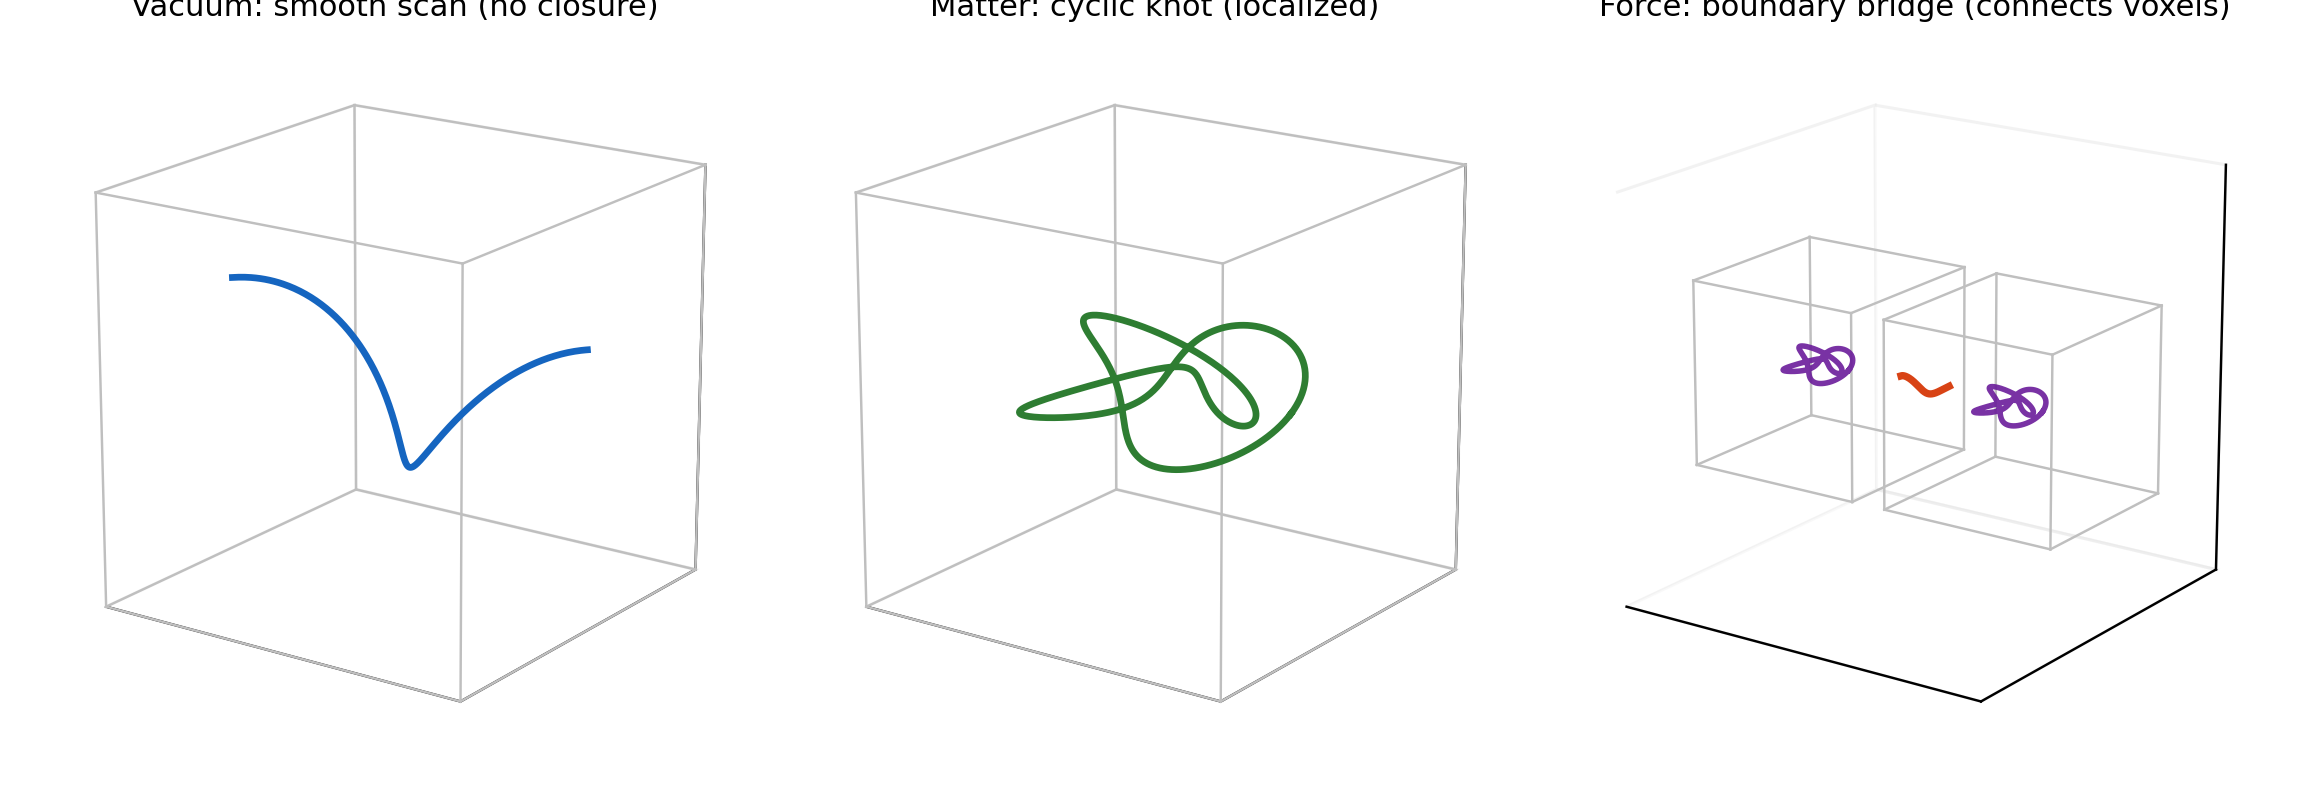
\includegraphics[width=\textwidth]{figures/hilbert_knot_triptych}
\caption{Conceptual triptych (interface picture). \emph{Left: Vacuum.} Below the 6-DoF anchor, a scan segment can be stable as a symbolic word yet remains sub-admissible for localized rigid-frame display; it is therefore treated as a non-local background (sub-geometric vacuum). \emph{Middle: Matter (cyclic).} At the $m=6$ anchor, stability can self-close into localized recurrent patterns; at the minimal anchor $(m,n)=(6,3)$ the stable sector obeys $64\to 21$ with a canonical cyclic/boundary split $21=18\oplus 3$. \emph{Right: Force (boundary).} Boundary-type patterns connect neighboring voxels/sites and are interpreted as interaction carriers enforcing cross-site consistency. This figure is a schematic geometric intuition and does not enter the theorem-level folding statements, which are formulated in finite readout language.}
\label{fig:hilbert_knot_triptych}
\end{figure}

\paragraph{The scan (1D).}
One may picture the readout as an extremely thin ``luminous thread'' whose order is fixed by the unitary scan: the observer sees only a time-ordered sequence of windowed binary words.

\paragraph{The fold (local compression).}
Once a locality dictionary is chosen, a single window must encode enough independent distinctions to be displayed as a localized object in that dictionary.
Under the minimal two-bin-per-DoF convention, this creates a geometric bottleneck at $m=6$ in $3$D: the readout must fold its local patterning to supply a coarse position--orientation frame.

\paragraph{The lock (closure vs.\ bridge).}
At the interface level, cyclic closure (a local recurrence) is interpreted as a fermion-like localized excitation, while boundary-type connectivity between neighboring sites is interpreted as a boson-like carrier that transmits readout constraints across space.
The subsequent sections make these statements auditable by fully explicit finite constructions at $(m,n)=(6,3)$ and by closed protocol-level interfaces.


